\chapter{Code Excerpts and Manual Processes}

The function in Listing \ref{fig:appendix-import-geometry-nodes} imports a dummy object containing the Geometry Nodes in the procedural graphics library. See Section \ref{sec:save-restore-blender-geometry}.
\begin{lstlisting}[language=python,caption={Geometry Nodes - Import Function},label={fig:appendix-import-geometry-nodes}]
def import_geometry_cube(blend_path):
    cube = blend_append_object(blend_path, GEOMETRY_DUMMY_CUBE_NAME)
    cube.select_set(True)
    cube.hide_render = True
    cube.hide_viewport = True
\end{lstlisting}


This functions in Listings \ref{fig:appendix-export-main-geometry-nodes}, \ref{fig:appendix-export-first-step-geometry-nodes} and \ref{fig:appendix-export-second-step-geometry-nodes}  compile and export a Geometry Nodes Library. See Section \ref{sec:save-restore-blender-geometry}.

\begin{lstlisting}[language=python,caption={Geometry Nodes - Export - Main Function},label={fig:appendix-export-main-geometry-nodes}]
def save_geometry(original_path, destination_path, skip_if_missing=True):
    if skip_if_missing and not pathlib.Path(original_path).is_file():
        return
    temp_path = GEOMETRY_TMP_FILE
    p = Process(target=_save_geometry_1, args=(original_path, temp_path, skip_if_missing))
    p.start()
    p.join()
    assert p.exitcode == 0

    p = Process(target=_save_geometry_2, args=(temp_path, destination_path, skip_if_missing))
    p.start()
    p.join()
    assert p.exitcode == 0
    try:
        os.unlink(temp_path)
    except Exception:
        pass
\end{lstlisting}


\begin{lstlisting}[language=python,caption={Geometry Nodes - Export - First Step},label={fig:appendix-export-first-step-geometry-nodes}]
def _save_geometry_1(original_path, destination_path, skip_if_missing=True):
    if skip_if_missing and not pathlib.Path(original_path).is_file():
        return

    scene = kb.Scene(resolution=(settings.RESOLUTION_X, settings.RESOLUTION_Y),
                     frame_start=1, frame_end=settings.MAX_FRAMES)
    renderer = Blender(
        scene, custom_scene=original_path, custom_scene_shading=True,
        adaptive_sampling=True, samples_per_pixel=settings.SAMPLES_PER_PIXEL,
    )
    pre_init_blender(renderer)
    cube_name = GEOMETRY_DUMMY_CUBE_NAME
    for obj in bpy.data.objects:
        if obj.name == GEOMETRY_DUMMY_CUBE_NAME:
            bpy.data.objects.remove(obj, do_unlink=True)

    scene += kb.Cube(name=cube_name, scale=(1, 1, 1), position=(0, 0, 0))

    with make_active_object(cube_name) as cube:
        cube.hide_render = True
        cube.hide_viewport = True

        already_added = set()
        for node_group in bpy.data.node_groups:
            # for each landmap item, set Geometry modifier
            if node_group.name in already_added:
                continue
            already_added.add(node_group.name)
            mod = cube.modifiers.new('geometry_wrapper_' + node_group.name, 'NODES')
            mod.node_group = bpy.data.node_groups[node_group.name]

        # immediately delete the created objects, since we *really* only want the cube
        for obj in bpy.data.objects:
            if obj.name != GEOMETRY_DUMMY_CUBE_NAME:
                bpy.data.objects.remove(obj, do_unlink=True)
            else:
                log.info('KEEP %s', obj.name)

    save_blend(renderer, destination_path)
\end{lstlisting}



\begin{lstlisting}[language=python,caption={Geometry Nodes - Export - Second Step},label={fig:appendix-export-second-step-geometry-nodes}]
def _save_geometry_2(original_path, destination_path, skip_if_missing=True):
    if skip_if_missing and not pathlib.Path(original_path).is_file():
        return

    scene = kb.Scene(resolution=(settings.RESOLUTION_X, settings.RESOLUTION_Y),
                     frame_start=1, frame_end=settings.MAX_FRAMES)
    renderer = Blender(scene, adaptive_sampling=True, samples_per_pixel=settings.SAMPLES_PER_PIXEL)
    pre_init_blender(renderer)
    import_geometry_cube(original_path)
    save_blend(renderer, destination_path)
\end{lstlisting}


The code in Listing \ref{fig:camera-path-interpolation} implements camera path interpolation as part of the scene setup process. See Section \ref{sec:rendering} for more details.

\begin{lstlisting}[language=python,caption={Camera Path Interpolation},label={fig:camera-path-interpolation}]
    anim_distance = (settings.MAX_FRAMES / settings.SIMULATION_FPS) * settings.CAMERA_ANIMATION_SPEED_M_S * 2 + 500
    animation_path = 'rails_center'
    with make_active_object(animation_path):
        path_vertices = [
            (d.index, (d.co.xyz.to_tuple()))
            for d in bpy.context.active_object.data.vertices
            if math.sqrt(
                d.co.xyz.to_tuple()[0]**2 + d.co.xyz.to_tuple()[1]**2
            ) < anim_distance
        ]
    index_count = [
        i for i, (x, y) in enumerate(
            zip([a[0] for a in path_vertices[:-1]],
                [a[0] for a in path_vertices[1:]])
        ) if x + 1 != y
    ]
    index_count = [0] + index_count + [len(path_vertices)]
    index_count = {index_count[k]: index_count[k + 1] - index_count[k]
                   for k in range(0, len(index_count) - 1)}
    start_idx, run_len = max(index_count.items(), key=lambda t: (t[1], random.random()))
    path_point = [path_vertices[k][1]
                  for k in range(1 + start_idx, start_idx + run_len + 1)
                  if k < len(path_vertices)]

    def _3d_dist(point, next_point):
        return math.sqrt((point[0] - next_point[0])**2 + (point[1] - next_point[1])**2 + (point[2] - next_point[2])**2)
    def _add_nan(points, avg_dist=1):
        log.info('adding NaN to %s points, interp dist %s', len(points), avg_dist)
        for point_id in range(0, len(points) - 1):
            point = points[point_id]
            next_point = points[point_id + 1]
            next_point_dist = _3d_dist(point, next_point)
            yield point
            yield from [(numpy.nan, numpy.nan, numpy.nan)] * int(next_point_dist / avg_dist)
        yield points[-1]

    start_to_end_dist = _3d_dist(path_point[0], path_point[-1])
    path_point = pandas.DataFrame(_add_nan(path_point, settings.CAMERA_ANIMATION_SPEED_M_S / settings.SIMULATION_FPS))
    path_point = path_point.interpolate(method='linear', limit_area='inside')
    path_point = [tuple(t[1]) for t in path_point.iterrows()]
    assert len(path_point) > settings.MAX_FRAMES
\end{lstlisting}

\newpage

Figure \ref{fig:manual-download-geo} describes the steps required to manually obtain geographic data using the GIS plugin. See more details in Section \ref{sec:dowonload-geo-data}.


\begin{figure}[H]
\begin{tabular}{ccc}

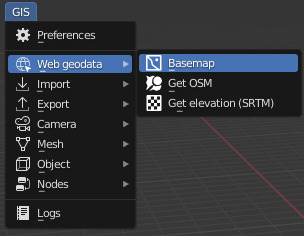
\includegraphics[width=42mm]{src/img/manual-download/1-get-basemap.jpg} &
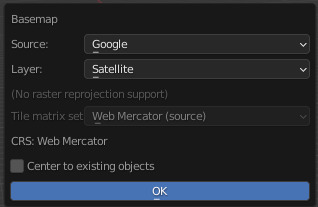
\includegraphics[width=42mm]{src/img/manual-download/2-choose-sat.jpg} &
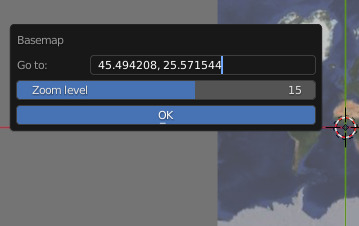
\includegraphics[width=42mm]{src/img/manual-download/3-choose-gps-zoom.jpg} \\
  (a) Open Base Map Form &  
  (b) Choose Satellite Provider &   
  (c) Choose Location and Zoom \\
  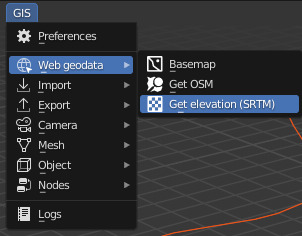
\includegraphics[width=42mm]{src/img/manual-download/4-get-alt.jpg} &
  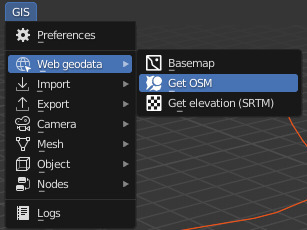
\includegraphics[width=42mm]{src/img/manual-download/5-get-osm.jpg} &
  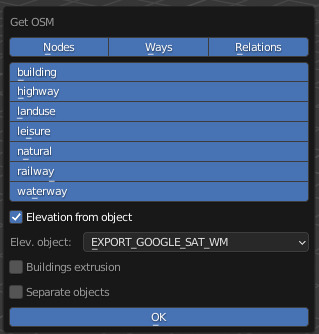
\includegraphics[width=42mm]{src/img/manual-download/6-osm-settings.jpg} \\
  (d) Obtain Altitude Data &   
  (e) Open OSM Form &          
  (f) Choose OSM Data \\
  \multicolumn{3}{c}{ 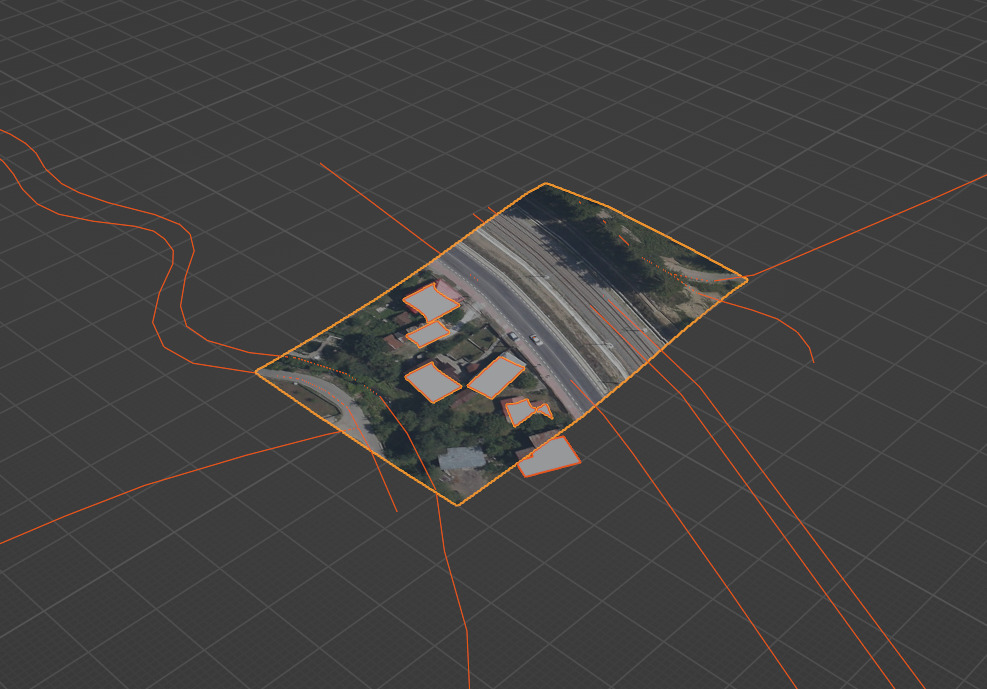
\includegraphics[width=130mm]{src/img/manual-download/7-end-result.jpg} }  \\ 
  \multicolumn{3}{c}{ (g) Save End Result }
 
\end{tabular}
\caption{Manual Process for Downloading Geographical Data}
\label{fig:manual-download-geo}
\end{figure}
